\documentclass[a4paper,10pt]{scrbook}
\usepackage{fontspec}
\usepackage[ngerman]{babel}
\usepackage{graphicx}
\usepackage{makeidx}
\usepackage{natbib}
\makeindex
\usepackage[colorlinks]{hyperref}
\providecommand{\tightlist}{%
\setlength{\itemsep}{0pt}\setlength{\parskip}{0pt}}

\begin{document}

Some text without meaning; really? with an image

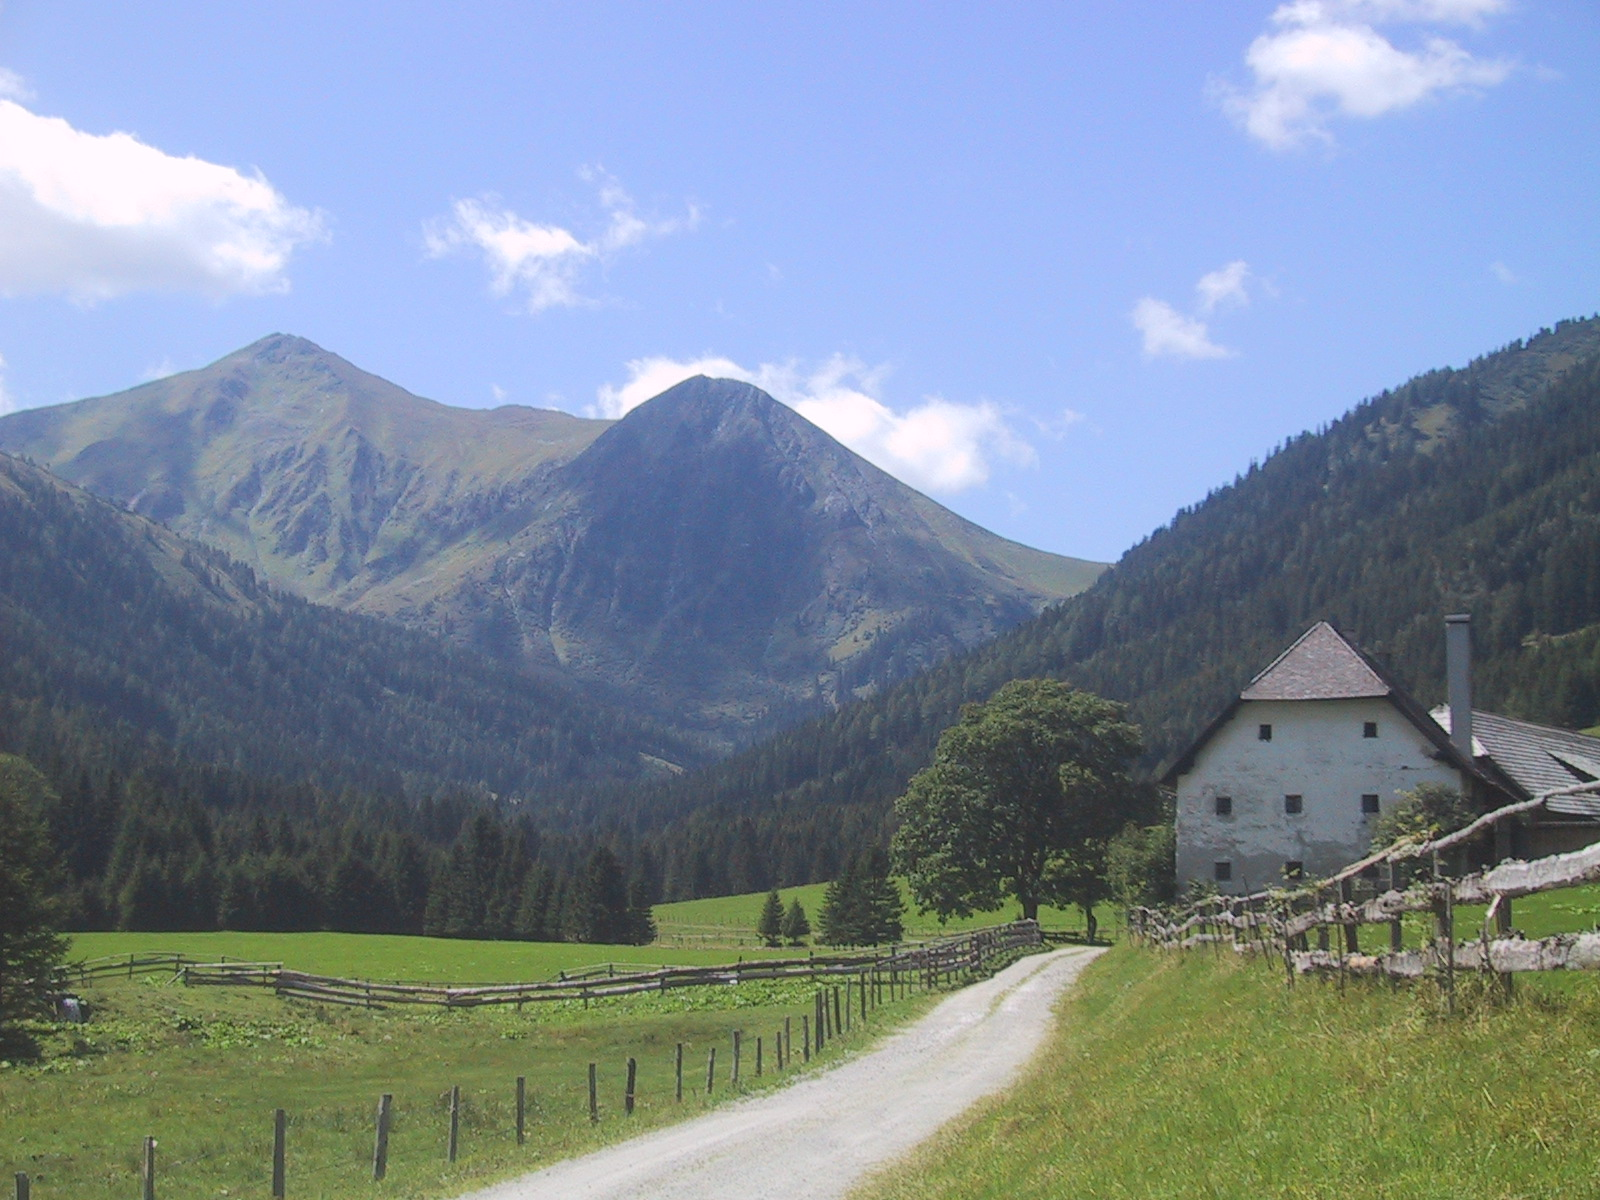
\includegraphics{/home/frank/Workspace11/ssg/docs/site/dough/resources/img/120-2026_IMG.JPG}

absolute statt relative path "/resources/img/120-2026\_IMG.JPG" An
example post. postwk but in blog - not in SubBlog with some additional
text which is always changed

addition


\printindex
\end{document}
